\documentclass[12pt,letterpaper]{article}
\usepackage{listings}
\usepackage{graphicx}
\usepackage[table,xcdraw]{xcolor}
\RequirePackage{xcolor}
\definecolor{tecAzul}{cmyk}{1,0.91,0.33,0.25} % según manual de imagen 2016
\definecolor{tecRojo}{cmyk}{0,0.9,0.86,0}     % según manual de imagen 2016

\renewcommand{\familydefault}{\sfdefault}
\usepackage{amsmath} % for the equation* environment
\usepackage{mwe}
\usepackage{graphicx}
\usepackage[spanish]{babel}
\usepackage{multirow}
\usepackage{titlesec}
\titleformat*{\section}%
{\normalfont\Large\bfseries\color{tecAzul}}
\titleformat*{\subsection}%
{\normalfont\large\bfseries\color{tecAzul}}


\usepackage[tmargin=2cm,bmargin=2cm,lmargin=2.5cm,rmargin=2.5cm]{geometry}
\usepackage{textpos}
\usepackage{tikz}
\usepackage{pgfplots}
\usepackage{pgf}

\usepackage[margin=1cm]{caption}

\usepackage{hyperref}

%
% paragraph layout
%
\parindent0em                           % indentation width of first line
\parskip1.3ex                           % space between paragraphs


\newcommand{\EstudianteA}{David F. Duarte Sánchez}

\pgfplotsset{compat=1.17}



\usepackage{listings}
\usepackage{xcolor}

\definecolor{codegreen}{rgb}{0,0.6,0}
\definecolor{codegray}{rgb}{0.5,0.5,0.5}
\definecolor{codepurple}{rgb}{0.58,0,0.82}
\definecolor{backcolour}{rgb}{0.95,0.95,0.92}

\lstdefinestyle{mystyle}{
    backgroundcolor=\color{backcolour},   
    commentstyle=\color{codegreen},
    keywordstyle=\color{magenta},
    numberstyle=\tiny\color{codegray},
    stringstyle=\color{codepurple},
    basicstyle=\ttfamily\footnotesize,
    breakatwhitespace=false,         
    breaklines=true,                 
    captionpos=b,                    
    keepspaces=true,                 
    numbers=left,                    
    numbersep=5pt,                  
    showspaces=false,                
    showstringspaces=false,
    showtabs=false,                  
    tabsize=2
}

\lstset{style=mystyle}



\begin{document}
	
\graphicspath{{./}{./fig/}}

%-------------------------- Title section -------------------------------------%

%
\begin{textblock}{10}[0,0](-0.5,0)
	\large Escuela de Ingeniería Electrónica \\ 
	EL5617 Trabajo Final de Graduación \\
\end{textblock}

%
\begin{textblock}{10}[0,0](2.6,-0.35)
	\begin{flushright}
		
\includegraphics[scale=0.8]{Firma_TEC-4.pdf}
	\end{flushright}
\end{textblock}

%% Title %%
\begin{center}
	\vspace{70mm}
	{\large\color{tecRojo} Trabajo Final de Graduación}
	\par\vspace{8mm}
	{\Large\bf\color{tecAzul}{Bitácora de Trabajo - Entrega 5}}
	\par\vspace{100mm}
	{{\EstudianteA \\ II Semestre 2024} 
	\vspace{8mm}}
\end{center}

\newpage
%------------------------------------------------------------------------------%

\renewcommand{\baselinestretch}{1.1}    % line spacing

%------------------------------------------------------------------------------%

\section{Semana 10}
\subsection{Corrección de Tesis}

\bf{Fecha de trabajo:} 20/09/2024.\\
\bf{Objetivo:} Compilacion y generacion del caso de uso por medio del flujo de trabajo propuesto.

\begin{table}[h!]
    \resizebox{\textwidth}{!}{%
    \begin{tabular}{|l|}
        \hline
        \hline
        \multicolumn{1}{|c|}{Reporte de   actividades} \\ \hline
        \hline
        -Generación del flujo de trabajo para el caso de uso seleccionado, en este caso como es \\
        una prueba de concepto se selecciona la implementación de un filtro simple, esto mediante el \\
        uso del bloque de simulink denominado sine wave, una suma y una función de transferencia,\\
        esto con el objetivo de demostrar la correcta implementación del modelo generado en matlab en \\
        código C, la compilación en el sistema linux orientado al procesador arm y la implementación en\\
        la tarjeta de desarrollo. \\ \hline

        -Creación de diagramas para el capítulo 4, con el objetivo de establecer un flujo más claro para el \\
        lector, los diagramas elaborados se adjuntan en las Figuras \ref{fig:diagrama_general_proyecto} , \ref{fig:flujo_linux}, \ref{fig:Simulink_coder}.\\ \hline

        -Documentación del capítulo 4 con los pasos específicos que se siguieron desde la generación del caso \\
        de uso en simulink como la compilación e implementación del mismo en linux, pasando por el compilador \\
        de arm en linux y la generación de la capa. \\\hline
    \end{tabular}}
\end{table}


\begin{figure}[h!]
    \centering
    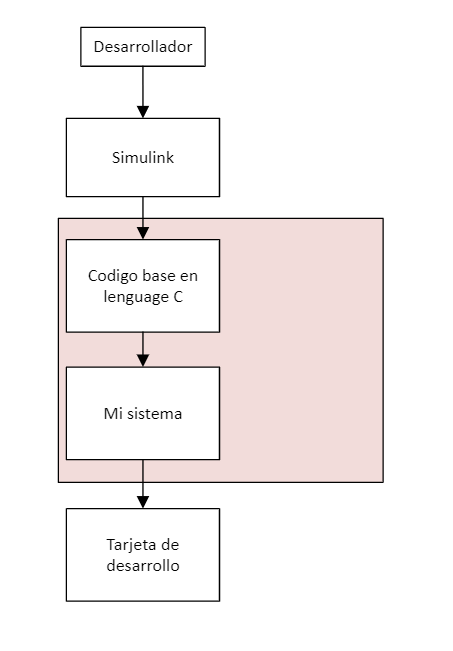
\includegraphics[width=0.8\textwidth]{images/diagrama1.png}
    \caption{Diagrama general del proyecto}
    \label{fig:diagrama_general_proyecto}
\end{figure}

  \begin{figure}[h!]
    \centering
    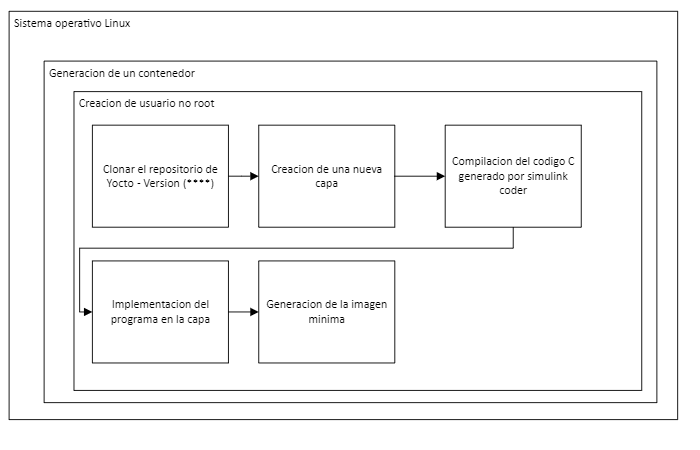
\includegraphics[width=0.8\textwidth]{images/diagrama2.png}
    \caption{Flujo Linux}
    \label{fig:flujo_linux}
  \end{figure}

  \begin{figure}[h!]
    \centering
    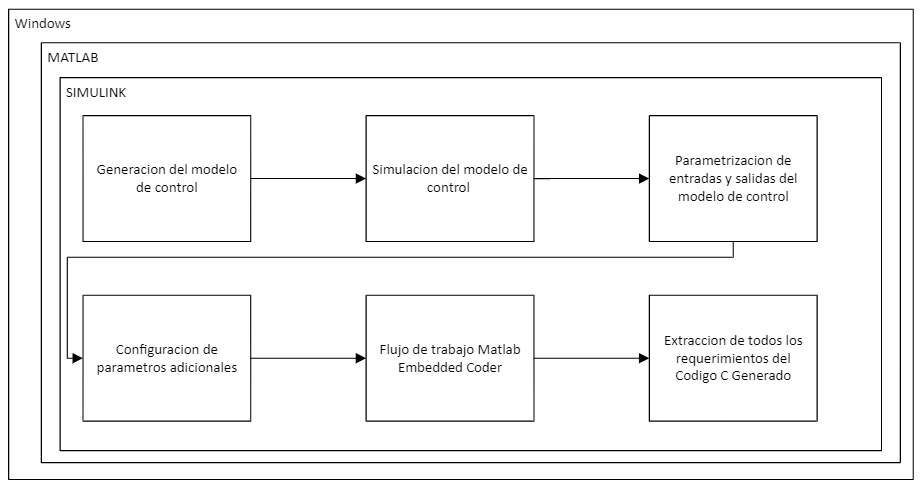
\includegraphics[width=0.8\textwidth]{images/diagrama3.png}
    \caption{Flujo Simulink Coder}
    \label{fig:Simulink_coder}
  \end{figure}

%\bibliography{bibliografia_consultada}
%\bibliographystyle{plain}
\end{document}